\documentclass{article}
\usepackage{v-problem}
\vgeometry

\begin{document}
\vtitle[ELECTROSTATICS]

\def\pn{04}
\def\book{Irodov}
\def\page{105}
\def\gdrive{https://drive.google.com/drive/folders/1ghKpAochsTlnJnyBm5xfABudOO0LkPbI?usp=share_link}

\def\question{
Two small equally charged spheres, each of mass $m$, are suspended from the same point by silk threads of length $l$. The distance between the spheres $x \ll l$. Find the rate $\d{q}/\d{t}$ with which the charge leaks off each sphere if their approach velocity varies as $v=a/\sqrt{x}$, where $a$ is a constant.
}

\vspace*{\fill}
\begin{tikzpicture}
	\node[qnumber] (n) at (0, 0)[scale=2] {$\pn.$};
	\node[question] (q) [right=2mm of n.east] {\question};
	\tzline[divider]<-0.125, 0> (q.north west)(q.south west);
	\node[format] (f) at  (q.south east){[\book \quad \page]};
\end{tikzpicture}	
\vspace*{\fill}

\begin{center}
\begin{tikzpicture}
\def\x{0.5}
\tzcoor*(0, 0)(O){$O$}[a]
\tzcoor*($(O)+(-\x, -3)$)(Q1){$m, q$}[bl](6pt)
\tzcoor*($(O)+(\x, -3)$)(Q2){$m, q$}[br](6pt)
	\tzline(O)(Q1){$l$}[ml]
	\tzline(O)(Q2){$l$}[mr]
	\tzline[|<->|]<0, -0.5>(Q1)(Q2){$x$}[mb]
\end{tikzpicture}
\end{center}
\vspace*{\fill}
\pagebreak

\vtitle[\texttt{Solution}]
\begin{center}

\begin{tikzpicture}
\def\l{1.5}
\tzcoor*(0, 0)(Q)(8pt)
	\tzline+[->](Q)(60:\l){$T$}[a]
	\tzline+[->](Q)(180:\l){$F_e$}[l]
	\tzline+[->](Q)(90:\l){$T\cos\theta$}[a]
	\tzline+[->](Q)(0:\l){$T\sin\theta$}[r]
	\tzline+[->](Q)(270:\l){$mg$}[b]
	\tzanglemark(60:1)(Q)(90:1){$\theta$}
	
\begin{scope}[xshift=6cm, yshift=\l cm]
\def\x{1.5}
\tzcoor*(0, 0)(O){$O$}[a]
\tzcoor*($(O)+(-\x, -3)$)(Q1){$m, q$}[bl](6pt)
\tzcoor*($(O)+(\x, -3)$)(Q2){$m, q$}[br](6pt)
	\tzline(O)(Q1){$l$}[ml]
	\tzline(O)(Q2){$l$}[mr]
	\tzline[|<->|]<0, -0.5>(Q1)(Q2){$x$}[mb]
	\tzanglemark(Q1)(O)($(O)+(0,-1)$){$\theta$}
	\tzline+[dashed](O)($(Q1)!0.5!(Q2)$)
	\tzline[dashed](Q1)($(Q1)!0.5!(Q2)$)
\end{scope}
\end{tikzpicture}
\end{center}

\addtolength{\jot}{2ex}
\begin{align*}
\intertext{From the left diagram}
T\cos\theta &= mg\\
T\sin\theta &= F_e 
\end{align*}

\begin{align}
\tan\theta &= \dfrac{F_e}{mg}
\end{align}

\pagebreak
\begin{align*}
\intertext{From the right diagram}
\tan\theta &= \dfrac{x/2}{\sqrt{l^2-\left(\dfrac{x}{2}\right)^2}}\\
\intertext{As $x\ll l$}
	&\approx \dfrac{x}{2l}
\end{align*}

\begin{align}
\tan\theta &= \dfrac{x}{2l}
\end{align}

\begin{align*}
\intertext{From equation (1) and (2)}
\dfrac{F_e}{mg} &= \dfrac{x}{2l}\\
\dfrac{1}{4\pi\varepsilon_0} \cdot \dfrac{q^2}{x^2} &= \dfrac{mgx}{2l}
\end{align*}
\begin{align}
q^2 &= \dfrac{2\pi\varepsilon_0 mgx^3}{l}
\end{align}
\pagebreak

\begin{align*}
\intertext{Now differentiate equation (3) w.r.t. time}
2q\dfrac{\d{q}}{\d{t}} &= \dfrac{2\pi\varepsilon_0 mg}{l}3x^2\dfrac{\d{x}}{\d{t}}\\[5mm]
\intertext{From equation (3), $q=\sqrt{\dfrac{2\pi\varepsilon_0 mg x^3}{l}}$}
\intertext{Approach velocity, $v=\dfrac{\d{x}}{\d{t}}=\dfrac{a}{\sqrt{x}}$}\\
	\sqrt{\dfrac{2\pi\varepsilon_0 mg x^3}{l}} \times \dfrac{\d{q}}{\d{t}} &= \dfrac{\pi\varepsilon_0 mg}{l}3x^2 \dfrac{a}{\sqrt{x}}\\[5mm]
	\Aboxed{\dfrac{\d{q}}{\d{t}} &= \dfrac{3a}{2} \sqrt{\dfrac{2\pi\varepsilon_0 mg}{l}}} \ans
\end{align*}

\pagebreak

\vspace*{\fill}
\begin{center}
	\fbox{\qrcode[height=2cm]{\gdrive}}
\end{center}
\vspace*{\fill}

\end{document}
